\chapter{有心力：行星与卫星}\label{ch:b1:central-forces}

三十一颗卫星每天绕地球两圈，每一颗都是一台时钟
与一部电台；一部手机若能收到其中四颗的信号，
便能把自己的位置精确到几米之内。哈雷彗星朝太阳下落
三十八年，在几周之内绕太阳掠过，
随后又远离太阳飞去三十八年。一个飞向火星的探测器，
以恰好的速率离开地球，使其轨道刚好与火星轨道相切。
这一切运动都是一个物体在受到
指向某一固定点、与距离平方成反比的力吸引时所作的运动，
并且全部可由两个守恒量——能量与角动量——以及一个新思想，
即有效势，推出。本章将推导轨道的形状与速率、
开普勒三定律，以及把卫星送到所需位置的
计算。

\section{有心保守力}

\begin{definition}[有心力；有心保守力]\label{def:b1:central-forces:central}
\index{有心力}\index{有效势}
若力以 $O$ 为中心，且始终沿 $\vect{OM}$ 的方向，
即 $\vect F = F(M)\,\vect e_r$，则称它是\emph{有心的}。若其大小只依赖于 $r = OM$，
则称它为\emph{有心保守的}，即 $\vect F =
F(r)\,\vect e_r$，由势能 $E_p(r)$ 导出，且满足
$F(r) = -\dd E_p/\dd r$.
\end{definition}

\begin{theorem}[有心保守力下的运动]\label{thm:b1:central-forces:reduction}
\index{面积定律}
质量为 $m$ 的质点只受一个有心保守力作用：
\begin{enumerate}
  \item 保持其角动量 $\vect L_O$ 不变；其运动是平面的，且
        在该平面内的极坐标下，$r^2\dot\theta = C$ 为常量
        （面积定律，见\cref{cor:b1:angular-momentum:central}）；
  \item 保持机械能 $E_m = \tfrac12 m(\dot r^2 + r^2\dot\theta^2)
        + E_p(r)$，可写为
        \[
        E_m = \tfrac12 m\dot r^2 + E_{p,\mathrm{eff}}(r), \qquad
        E_{p,\mathrm{eff}}(r) = E_p(r) + \frac{mC^2}{2r^2} = E_p(r) + \frac{L^2}{2mr^2} .
        \]
\end{enumerate}
因此径向运动即为一维质点在
\emph{有效势} $E_{p,\mathrm{eff}}$ 中的运动：径向转折点是
方程 $E_{p,\mathrm{eff}}(r) = E_m$ 的根，若运动被夹在其中两根之间，则是束缚的，
而若 $r$ 恰位于 $E_{p,\mathrm{eff}}$ 的
极小值处，则为圆周运动。
\end{theorem}

\begin{proof}
第 1 部分由\cref{cor:b1:angular-momentum:central}即得。该力是
保守力，且无其他力作用，故 $E_m$ 守恒；在平面内，
有 $v^2 = \dot r^2 + r^2\dot\theta^2$，且 $r^2\dot\theta^2 = C^2/r^2$。
项 $mC^2/2r^2$，即角向运动的动能，在径向问题中起到
排斥性的\emph{离心势垒}作用，可用
可用\cref{ch:b1:work-and-energy}中的一维分析方法处理。
\end{proof}

\section{牛顿引力}

\begin{definition}[万有引力]\label{def:b1:central-forces:gravitation}
\index{万有引力}\index{重力势能}
质量为 $M$ 的质点位于 $O$ 处，吸引质量为 $m$、位于 $M$ 处的质点，其关系为
\[
\vect F = -\frac{GMm}{r^2}\,\vect e_r, \qquad E_p = -\frac{GMm}{r} \quad (E_p \to 0 \text{ 在无穷远处}),
\]
其中 $G = \qty{6.67e-11}{N.m^2/kg^2}$。球对称物体对其外部的吸引，
等同于将其质量集中于球心（在本阶段不加证明地承认；
这是\cref{ch:b1:electrostatics-gauss}中高斯定理的推论）。
\end{definition}

\begin{proposition}[引力的有效势]\label{prop:b1:central-forces:effective}
\index{离心势垒}\index{圆轨道}
对于 $E_p = -GMm/r$，
\[
E_{p,\mathrm{eff}}(r) = -\frac{GMm}{r} + \frac{L^2}{2mr^2}
\]
有效势趋于 $+\infty$（$r \to 0$，$L \neq 0$），在无穷远处趋于 $0^-$，
有唯一的极小值，位于 $r_c = L^2/GMm^2$ 处，其值为 $-G^2M^2m^3/2L^2$。
由此可得：$E_m < 0$——运动是束缚的，位于极小与极大半径之间（近心点与远心点）；
$E_m \geq 0$——运动是非束缚的，物体自无穷远来，
并返回无穷远；$E_m$ 等于极小值时——为
半径为 $r_c$ 的圆轨道。
\end{proposition}

\begin{proof}
极限由观察可得；$E_{p,\mathrm{eff}}' = GMm/r^2 - L^2/mr^3 = 0$ 在
$r_c$ 处成立；代入即可。圆轨道情形即 $\dot r = 0$ 恒成立，
这只可能发生在极小值处。
\end{proof}

\begin{omfigure}
\begin{tikzpicture}
\begin{axis}[omaxis, axis x line=bottom, axis y line=left, width=10.5cm, height=6cm, xlabel={$r/r_c$}, ylabel={$E_{p,\mathrm{eff}}$},
    xlabel style={at={(axis description cs:0.5,-0.06)}, anchor=north},
    xmin=0, xmax=6, ymin=-1.2, ymax=1.2, xtick={1,2,3,4,5}, ytick={-1,0,1}, yticklabels={$-\frac{GMm}{2r_c}$,$0$,}]
  \addplot[omDef, thick, domain=0.36:6, samples=300] {-2/x + 1/x^2};
  \addplot[omExo, dashed, domain=0:6, samples=2] {0};
  \addplot[omThm, dashed, domain=0:6, samples=2] {-0.5};
  \addplot[omProp, dashed, domain=0:6, samples=2] {0.4};
  \draw[Stealth-Stealth, omThm] (axis cs:0.586,-0.5) -- (axis cs:3.41,-0.5);
  \node[omThm, font=\footnotesize, above] at (axis cs:2.0,-0.48) {$E_m < 0$：椭圆};
  \node[omProp, font=\footnotesize, above] at (axis cs:3.5,0.42) {$E_m > 0$：双曲线};
  \node[omExo, font=\footnotesize, above] at (axis cs:4.8,0.02) {$E_m = 0$：抛物线};
  \fill[omDef] (axis cs:1,-1) circle (1.5pt); \node[omDef, font=\footnotesize, right] at (axis cs:1.15,-1.0) {圆轨道};
  \node[font=\footnotesize, omDef] at (axis cs:0.9,0.8) {$\dfrac{L^2}{2mr^2}$};
  \node[font=\footnotesize, omDef] at (axis cs:5.2,-0.72) {$-\dfrac{GMm}{r}$};
\end{axis}
\end{tikzpicture}

{\small 牛顿引力的有效势：引力项 $-GMm/r$ 与
离心势垒项 $L^2/2mr^2$ 之和。能量为负时，径向运动
被限制在两个转折点之间（近心点、远心点）；
在极小值处轨道为圆形；能量为零或正时，
物体逃逸。}
\end{omfigure}

\begin{theorem}[圆轨道]\label{thm:b1:central-forces:circular}
\index{轨道速率}\index{开普勒第三定律}
在半径为 $r$、绕质量为 $M$ 的天体运行的圆轨道上：
\[
v = \sqrt{\frac{GM}{r}}, \qquad
T = 2\pi\sqrt{\frac{r^3}{GM}}, \qquad
E_m = -\frac{GMm}{2r} = -E_k = \tfrac12 E_p .
\]
特别地，对同一中心的所有圆轨道，$T^2/r^3 = 4\pi^2/GM$ 是相同的
（开普勒第三定律）。
\end{theorem}

\begin{proof}
匀速圆周运动需要向心力 $mv^2/r = GMm/r^2$；
$T = 2\pi r/v$；$E_k = \tfrac12 mv^2 = GMm/2r$ 及 $E_p = -GMm/r$。
\end{proof}

\begin{example}[三种轨道]\label{ex:b1:central-forces:orbits}
$GM_\oplus = \qty{3.99e14}{m^3/s^2}$。低轨道（$r = \qty{6770}{km}$，
高出地面 \qty{400}{km}）：$v = \qty{7.7}{km/s}$，$T = \qty{92}{min}$。地球静止轨道
（$T = \qty{86164}{s}$，一个恒星日）：$r = (GMT^2/4\pi^2)^{1/3} =
\qty{42200}{km}$，$v = \qty{3.1}{km/s}$。月球（$r = \qty{384000}{km}$）：
$T = \qty{27.4}{d}$——其向心加速度 $v^2/r =
\qty{2.7e-3}{m/s^2}$，在六十个地球半径处恰为 $g/3600$：平方反比
律，由牛顿本人检验。
\end{example}

\section{开普勒定律与轨道形状}

\begin{theorem}[牛顿场中的轨迹]\label{thm:b1:central-forces:conics}
\index{开普勒定律}\index{圆锥曲线}\index{椭圆（轨道）}\index{偏心率}
固定质量 $M$ 的场中，物体的轨迹为圆锥曲线，
且 $O$ 位于其一个焦点上：$E_m < 0$ 时为椭圆，$E_m = 0$ 时为抛物线，
$E_m > 0$ 时为双曲线。对于半长轴为 $a$ 的椭圆，
偏心率为 $e$：
\begin{itemize}
  \item （开普勒第一定律）力心位于焦点上；近心点和远心点
        分别位于 $r_p = a(1 - e)$ 和 $r_a = a(1 + e)$；
  \item （开普勒第二定律）面速度守恒（即面积定律）；
  \item （开普勒第三定律）周期满足 $T^2 = 4\pi^2a^3/GM$；
  \item 能量仅取决于 $a$，即 $E_m = -GMm/2a$，于是
        距离为 $r$ 处的速率由下式给出：
        \[
        v^2 = GM\left(\frac{2}{r} - \frac{1}{a}\right) .
        \]
\end{itemize}
\end{theorem}
\admitted

\begin{remark}[已证明与承认的内容]\label{rem:b1:central-forces:admitted}
开普勒第二定律与能量分类已在上文证明。关于
束缚轨道恰为以 $O$ 为焦点的椭圆，连同开普勒第三定律，
以及一般情形下的 $E_m = -GMm/2a$，需要对径向方程进行积分
（本科二年级分册中完成）；对圆轨道（$a = r$，
$e = 0$），各结论都归结为\cref{thm:b1:central-forces:circular}，
这正是此处可作的检验。关系式 $v^2 = GM(2/r - 1/a)$
在承认该能量公式的前提下，
由 $E_m = \tfrac12 mv^2 - GMm/r = -GMm/2a$ 可得。
\end{remark}

\begin{omfigure}
\begin{tikzpicture}[font=\small, x=1cm, y=1cm]
  % ellipse a=3, e=0.6, c=1.8, b=2.4 ; focus O at origin ; center at (-1.8,0)
  \draw[omDef, thick] (-1.8,0) ellipse (3 and 2.4);
  \fill (0,0) circle (1.8pt) node[below] {$O$};
  \fill (-3.6,0) circle (1.2pt) node[below] {$O'$};
  \draw[dashed] (-4.8,0) -- (1.2,0);
  \fill[omThm] (1.2,0) circle (1.6pt) node[below right] {$P$};
  \fill[omThm] (-4.8,0) circle (1.6pt) node[below left] {$A$};
  \draw[Stealth-Stealth, omExo] (-1.8,-2.6) -- (1.2,-2.6) node[midway, below] {$a$};
  \draw[Stealth-Stealth, omExo] (-1.8,0.1) -- (-1.8,2.4) node[midway, left] {$b$};
  \draw[Stealth-Stealth, omExo] (-1.8,0.45) -- (0,0.45) node[midway, above] {$c = ea$};
  \node[omThm, font=\footnotesize] at (0.7,0.8) {$r_p = a(1 - e)$};
  \node[omThm, font=\footnotesize] at (-3.4,0.8) {$r_a = a(1 + e)$};
  % hyperbola and parabola sketches on the right
  \begin{scope}[xshift=6.3cm]
  \fill (0,0) circle (1.8pt) node[below] {$O$};
  \draw[omProp, thick, domain=-1.55:1.55, samples=80, variable=\t] plot ({1.0*cosh(\t)-1.6},{1.2*sinh(\t)});
  \draw[omExo, thick, domain=-2.4:2.4, samples=80, variable=\y] plot ({0.5*\y*\y-2.6},{\y});
  \node[omProp, font=\footnotesize] at (0.0,2.9) {$E_m > 0$};
  \node[omExo, font=\footnotesize] at (-2.2,2.9) {$E_m = 0$};
  \end{scope}
\end{tikzpicture}

{\small 左图：绕焦点 $O$ 运行的椭圆轨道——半长轴
$a$，半短轴 $b$，焦距 $c = ea$；物体在
近心点 $P$ 处速率最大，远心点 $A$ 处速率最小。右图：双曲线（正能量）与
抛物线（零能量），二者绕同一焦点——即
彗星与探测器的非束缚轨道。}
\end{omfigure}

\begin{example}[哈雷彗星]\label{ex:b1:central-forces:halley}
近日点 \qty{0.586}{AU}，远日点 \qty{35.1}{AU}：$a = \qty{17.8}{AU}$，
$e = 0.967$，$T = \sqrt{17.8^3} = \qty{75}{years}$（开普勒第三定律以
天文单位和年为单位表示，其中对太阳有 $T^2 = a^3$）。
取 $GM_\odot = \qty{1.33e20}{m^3/s^2}$，则近日点速率为
$\sqrt{GM(2/r_p - 1/a)} = \qty{54}{km/s}$，远日点处为 \qty{0.9}{km/s}
——慢六十倍，符合面积定律的要求（$r_pv_p = r_av_a$）。
\end{example}

\section{卫星}

\begin{proposition}[逃逸速度；地球静止轨道]\label{prop:b1:central-forces:escape}
\index{逃逸速度}\index{地球静止轨道}
从质量为 $M$、半径为 $R$ 的天体表面出发，使物体到达无穷远的
最小发射速率为 $v_e = \sqrt{2GM/R} = \sqrt2\,v_c$，
其中 $v_c = \sqrt{GM/R}$ 为地面处的圆轨道速率：
对地球而言为 \qty{11.2}{km/s}。\emph{地球静止}卫星在赤道面内绕行，
周期等于地球的恒星日，轨道位于
$r = \qty{42200}{km}$ 处（距地面 \qty{35800}{km}）。
\end{proposition}

\begin{proof}
$E_m \geq 0$：$\tfrac12 mv_e^2 - GMm/R = 0$。取 $T = \qty{86164}{s}$，由开普勒第三定律。
\end{proof}

\begin{proposition}[霍曼转移]\label{prop:b1:central-forces:hohmann}
\index{霍曼转移}
要使卫星从半径为 $r_1$ 的圆轨道转移到
共面、半径为 $r_2 > r_1$ 的圆轨道，只需两次短暂点火：在 $r_1$ 处点火，
进入近地点为 $r_1$、远地点为 $r_2$ 的\emph{转移椭圆}
（$a = (r_1 + r_2)/2$），滑行半个周期，
再在 $r_2$ 处第二次点火，使轨道变为圆轨道：
\[
\Delta v_1 = \sqrt{\frac{GM}{r_1}}\left(\sqrt{\frac{2r_2}{r_1 + r_2}} - 1\right),
\qquad
\Delta v_2 = \sqrt{\frac{GM}{r_2}}\left(1 - \sqrt{\frac{2r_1}{r_1 + r_2}}\right),
\qquad
t = \pi\sqrt{\frac{(r_1 + r_2)^3}{8GM}} .
\]
\end{proposition}

\begin{proof}
由 $v^2 = GM(2/r - 1/a)$ 可求转移椭圆在 $r_1$ 与
$r_2$ 处的速率，减去圆轨道速率，再
\cref{thm:b1:central-forces:conics}可得半个周期。
\end{proof}

\begin{omfigure}
\begin{tikzpicture}[font=\small, x=1cm, y=1cm]
  \fill (0,0) circle (2.5pt) node[below left] {$O$};
  \draw[omDef, thick] (0,0) circle (1.0);
  \draw[omDef, thick] (0,0) circle (3.0);
  % transfer ellipse: perigee r1=1 at (1,0), apogee r2=3 at (-3,0): a=2, c=1, center (-1,0), b=sqrt(3)=1.732
  \draw[omThm, thick] (-1,0) ellipse (2 and 1.732);
  \fill[omThm] (1,0) circle (1.6pt); \fill[omThm] (-3,0) circle (1.6pt);
  \draw[-Stealth, omExo, very thick] (1,0) -- (1,1.0) node[right] {$\Delta v_1$};
  \draw[-Stealth, omExo, very thick] (-3,0) -- (-3,-0.8) node[left] {$\Delta v_2$};
  \node[omDef, font=\footnotesize] at (1.5,-1.2) {$r_1$};
  \node[omDef, font=\footnotesize] at (2.6,2.3) {$r_2$};
  \node[omThm, font=\footnotesize] at (-1.0,2.0) {转移椭圆};
  \draw[-Stealth, omThm] (-0.2,1.72) -- (-0.8,1.73);
\end{tikzpicture}

{\small 两圆轨道之间的霍曼转移：在内侧轨道上做第一次点火，
将远地点抬至 $r_2$；半个椭圆之后，
第二次点火抬高近地点——这是燃料最省的两次点火路径，并且
也是探测器飞往火星所用的路线。}
\end{omfigure}

\begin{example}[从低轨道到地球静止轨道]\label{ex:b1:central-forces:leogeo}
$r_1 = \qty{6770}{km}$, $r_2 = \qty{42200}{km}$: $\Delta v_1 = \qty{2.4}{km/s}$,
$\Delta v_2 = \qty{1.5}{km/s}$，滑行 \qty{5.3}{h}。总量
\qty{3.9}{km/s}，约为发射入低轨道所耗量的一半。通往高轨道的
“最后一英里”代价高昂，卫星为此须自带
发动机。
\end{example}

\begin{remark}[排斥中心]\label{rem:b1:central-forces:rutherford}
\index{卢瑟福散射}
对于排斥的平方反比力（两同号电荷，
见\cref{ch:b1:electrostatics-gauss}），有效势没有势阱：
每条轨迹都是双曲线：粒子接近、
被偏转后离开。把 $\alpha$ 粒子直接射向金原子核时，其
最近距离仅由能量决定，$E_k =
2Ze^2/4\pi\varepsilon_0 r_{\min}$——这是卢瑟福用以界定原子核大小的办法
（\cref{exo:b1:central-forces:11}）。
\end{remark}

\section{练习}

\begin{exercise}[$\star$]\label{exo:b1:central-forces:1}
国际空间站在 \qty{400}{km} 高度处绕地球运行
（$R_\oplus = \qty{6370}{km}$，$GM_\oplus = \qty{3.99e14}{m^3/s^2}$）。求其速率、
周期及乘员每天所见的日出次数。
\end{exercise}

\begin{exercise}[$\star$]\label{exo:b1:central-forces:2}
求地球静止轨道的半径与高度，由
恒星日 \qty{86164}{s} 出发，并求其轨道速率。
\end{exercise}

\begin{exercise}[$\star$]\label{exo:b1:central-forces:3}
求地球与月球的逃逸速度（$GM = \qty{4.90e12}{m^3/s^2}$，
$R = \qty{1740}{km}$）。月球为何没有大气层？
\end{exercise}

\begin{exercise}[$\star$]\label{exo:b1:central-forces:4}
火星 $a = \qty{1.524}{AU}$，木星 \qty{5.20}{AU}：由开普勒第三定律求
它们的公转周期；位于 \qty{30}{AU} 处（海王星）的天体，其周期为多少？
\end{exercise}

\begin{exercise}[$\star\star$]\label{exo:b1:central-forces:5}
求把 \qty{1000}{kg} 的物体从地面静止出发送入
国际空间站轨道所需的能量（忽略地球自转及空气阻力），
并与汽油的化学能（\qty{46}{MJ/kg}）相比较。
\end{exercise}

\begin{exercise}[$\star\star$]\label{exo:b1:central-forces:6}
哈雷彗星：近日点 \qty{0.586}{AU}，远日点 \qty{35.1}{AU}。
求 $a$、$e$、周期，以及近日点与远日点处的速率，
（$GM_\odot = \qty{1.33e20}{m^3/s^2}$，$\qty{1}{AU} = \qty{1.496e11}{m}$）。
\end{exercise}

\begin{exercise}[$\star\star$]\label{exo:b1:central-forces:7}
求从国际空间站轨道（\qty{6770}{km}）到
地球静止轨道（\qty{42200}{km}）的霍曼转移：两次点火的速度改变量、总量以及持续时间。
\end{exercise}

\begin{exercise}[$\star\star$]\label{exo:b1:central-forces:8}
证明 $E_{p,\mathrm{eff}}$ 的极小值位于 $r_c = L^2/GMm^2$，
并证明在其附近的小径向振动具有角频率
$\sqrt{GM/r_c^3}$——恰为轨道频率本身。这一结果对
略受扰动的圆轨道说明了什么？
\end{exercise}

\begin{exercise}[$\star\star$]\label{exo:b1:central-forces:9}
国际空间站上的宇航员处于漂浮状态。试用受力分析解释，
并求其所在高度处的 $g$ 值，
说明为何这与漂浮状态并不矛盾。
\end{exercise}

\begin{exercise}[$\star\star\star$]\label{exo:b1:central-forces:10}
牛顿的“月球检验”：计算月球的向心加速度，
所用数据为 $r = \qty{3.84e8}{m}$ 与 $T = \qty{27.3}{d}$，并与 $g(R/r)^2$ 比较。
由此得出结论。
\end{exercise}

\begin{exercise}[$\star\star\star$]\label{exo:b1:central-forces:11}
一个 $\alpha$ 粒子（$q = 2e$，$E_k = \qty{5.0}{MeV}$）沿直线射向
一个固定不动的金原子核（$Z = 79$）。利用能量守恒，
并取 $E_p = 2Ze^2/4\pi\varepsilon_0r$（$1/4\pi\varepsilon_0 = \qty{8.99e9}{SI}$），
求最近距离，并与原子核半径比较，
原子核半径约为 \qty{7}{fm}。要使粒子恰能接触原子核，需要多大能量？
\end{exercise}

\begin{exercise}[$\star\star\star$]\label{exo:b1:central-forces:12}
近地轨道上的卫星受残留大气作用而减速，其机械能随之减小。
利用 $E_m = -GMm/2r$ 与 $v = \sqrt{GM/r}$，证明此时卫星运动得\emph{更快}。
那么，能量去了哪里？
失去的势能中有多大比例转化为热量？
\end{exercise}

\begin{omfigure}
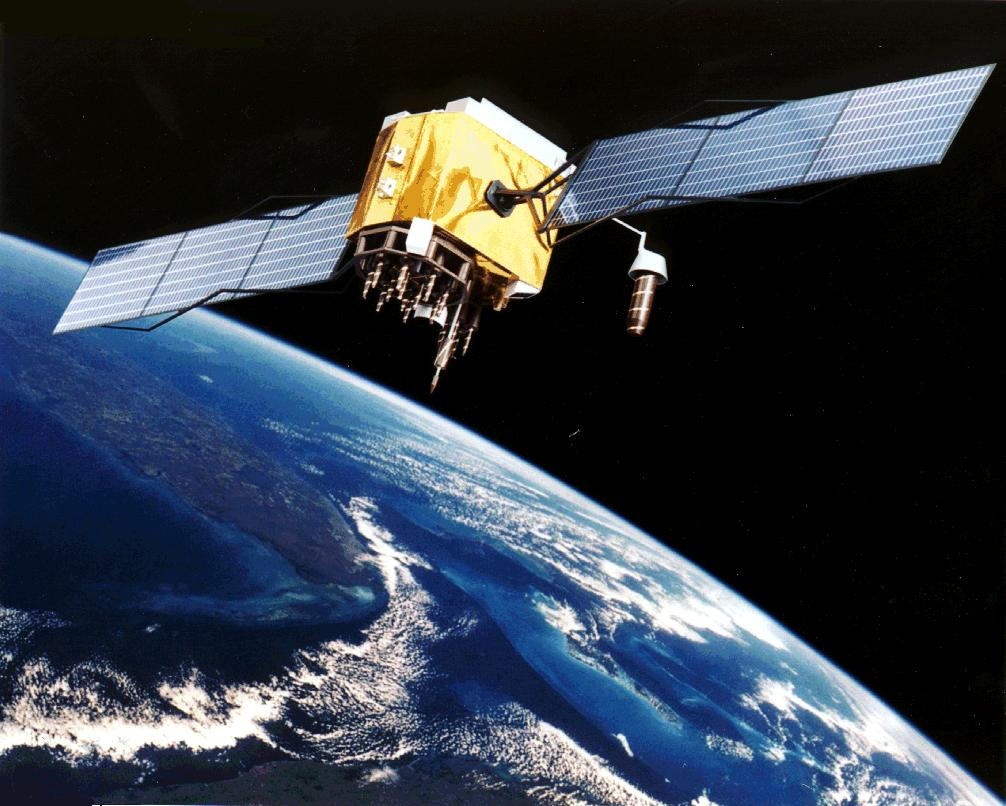
\includegraphics[width=0.46\linewidth]{images/book3/gps-satellite-nasa.jpg}

{\small 一颗 GPS 卫星（NASA 艺术家视角）：周末问题中 \qty{20200}{km} 高度的导航星座约有三十余颗卫星，每颗都是沿开普勒轨道运行的时钟。}
\end{omfigure}

\section{问题：告诉你身在何处的卫星}

\begin{problem}[{周末问题——位于两万千米高处的导航星座：
其轨道，以及抵达该轨道所需的燃料，
手机能看到多少颗卫星，
以及为何必须让它们的时钟走慢}]
\label{pb:b1:central-forces:1}
数据：$GM_\oplus = \qty{3.986e14}{m^3/s^2}$，$R_\oplus = \qty{6371}{km}$，
恒星日 \qty{86164}{s}，$c = \qty{2.998e8}{m/s}$。卫星
在圆轨道上绕地球运行，周期恰为半个恒星日。

\medskip
\noindent\textbf{第一部分——轨道。}
\begin{enumerate}
  \item 计算轨道半径与高度。
  \item 计算轨道速率。
  \item 计算卫星的加速度，并与
        地表处的 $g$ 作比较。
  \item 计算单位质量的机械能，
        以及其中的动能与势能部分。
  \item 为何选择半个恒星日，而不是半个太阳日？
        地面观测者会看到什么现象重复出现？
  \item 从卫星上看，地球圆面所张的角是多大？
  \item 将轨道半径与地球静止轨道的半径比较，哪一个更高，
        高出多少倍？
\end{enumerate}

\medskip
\noindent\textbf{第二部分——抵达轨道。}
\begin{enumerate}[resume]
  \item 从地表静止出发到达最终轨道时，每千克所需的能量
        （忽略空气与地球自转）。
  \item 运载火箭先到达 \qty{400}{km} 高的近地圆轨道，
        该处的速率是多少？
  \item 由该轨道到最终轨道的霍曼转移：两次点火的速度改变量
        及其总和。
  \item 转移的持续时间。
  \item 将两次点火速度改变量之和与近地轨道的逃逸速度比较，
        这次任务距离“离开地球”还有多远？
  \item 转移前，上面级与卫星的质量为 \qty{2000}{kg}；
        发动机的喷出速率为 \qty{3.0}{km/s}，
        由火箭方程 $\Delta v = u\ln(m_0/m_1)$ 可知，
        完成两次点火所需的推进剂为多少？
\end{enumerate}

\medskip
\noindent\textbf{第三部分——覆盖范围与时间。}
\begin{enumerate}[resume]
  \item 卫星可见的地面各点，应位于
        以地球–卫星连线为轴、半顶角为 $\theta$（$\cos\theta = R/r$）的圆锥之内。
        求 $\theta$，并求其覆盖地表的比例，
        即 $(1 - \cos\theta)/2$。
  \item 若 $24$ 颗卫星均匀分布，平均有多少颗可从某一点看到？
        平均能否满足定位所需的最少 $4$ 颗？
        这是否合理？
  \item 卫星位于天顶时，光从卫星到达地面的传播时间；
        位于地平线时的传播时间。
  \item 若要将接收机定位到 \qty{3}{m} 的精度，
        信号的计时精度应达到多少？
  \item 接收机自身的时钟是廉价石英钟，误差可达
        毫秒量级：为何需要四颗卫星而不是三颗？
  \item 卫星上的时钟是原子钟。给出经过一天后误差为 \qty{3}{m} 所需的
        相对稳定度。
\end{enumerate}

\medskip
\noindent\textbf{第四部分——简要的相对论修正。}
两种效应使卫星时钟相对地面时钟发生偏移：
（公式在本阶段不加证明地承认，取自本科三年级分册），运动使时钟变慢，变慢的比例为
$v^2/2c^2$；高度使时钟变快，变快的比例为 $GM(1/R - 1/r)/c^2$。
\begin{enumerate}[resume]
  \item 计算由速度引起的变慢量（以微秒每天计）。
  \item 计算由高度引起的变快量，以微秒
        每天计。
  \item 净效应，以及若不作修正每天造成的
        位置误差。
  \item 卫星时钟在发射前被设定为
        \qty{10.22999999543}{MHz}，而不是 \qty{10.23}{MHz}。验证这一设定
        能否抵消上述净效应。
  \item 实际轨道并非严格的开普勒轨道：请列举三种摄动，
        并说明系统如何应对。
  \item 总结这一链条：两条守恒定律、一条轨道、一个星座，
        以及一项无人能预料到的修正。
\end{enumerate}
\end{problem}
